\documentclass[tikz,border=2mm]{standalone}
\usepackage{tikz}
\usetikzlibrary{positioning}
\begin{document}
    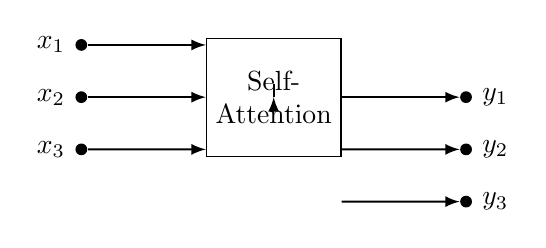
\begin{tikzpicture}[scale=0.8]
        \tikzset{layer/.style={draw,minimum width=1.5cm,minimum height=1.5cm}}
        \tikzset{dot/.style={circle,fill,inner sep=1.5pt}}
        \tikzset{vec/.style={draw,thick,-latex}}
        
        \node[dot,label=left:$x_1$] (x1) at (0,0) {};
        \node[dot,label=left:$x_2$,below=0.5cm of x1] (x2) {};
        \node[dot,label=left:$x_3$,below=0.5cm of x2] (x3) {};
        
        \node[layer,right=1.5cm of x2,align=center] (self-att) {Self-\\Attention};
        
        \node[dot,label=right:$y_1$,right=1.5cm of self-att] (y1) {};
        \node[dot,label=right:$y_2$,below=0.5cm of y1] (y2) {};
        \node[dot,label=right:$y_3$,below=0.5cm of y2] (y3) {};
        
        \foreach \i in {1,...,3} {
            \draw[vec] (x\i) -- (self-att.west |- x\i);
            \draw[vec] (self-att.east |- y\i) -- (y\i);
        }
        
        \draw[vec] (self-att) -- (self-att);
    \end{tikzpicture}
\end{document}
